% PLEASE USE THIS FILE AS A TEMPLATE
% Check file iosart2x.tex for more examples

% add. options: [seceqn,secthm,crcready,onecolumn]
\documentclass[aic]{iosart2x}

\usepackage[T1]{fontenc}
\usepackage[latin9]{inputenc}
\usepackage{array}
%\usepackage{url}
\usepackage{multirow}
\usepackage{graphicx}
%\usepackage{caption}
%\usepackage{subcaption}
%\captionsetup{compatibility=false}
\usepackage{verbatim}

\usepackage{tikz}
\usetikzlibrary{shapes,arrows,positioning,arrows.meta}

%\usepackage{babel}
\usepackage{listings}
\renewcommand{\lstlistingname}{Listing}

%\usepackage{dcolumn}
%\usepackage{endnotes}

%%%%%%%%%%% Put your definitions here

\newcommand{\eg}{\emph{e.g.}}
\newcommand{\ie}{\emph{i.e.}}
\newcommand{\etal}{\emph{et al.}}
\newcommand{\todo}[1]{\textcolor{red}{\bf [TODO: #1]}}
%\renewcommand{\todo}[1]{}
\newcommand{\yp}[1]{\textcolor{blue}{#1}}
\newcommand{\note}[1]{\textcolor{green}{[Note: #1]}}
\newcommand{\append}[1]{\textcolor{violet}{[Appendix?] #1}}
\newcommand{\zm}[1]{#1}
\newcommand{\hide}[1]{}
\newcommand{\figtitle}[1]{\textbf{#1}\par\medskip}
\renewcommand{\figtitle}[1]{}

%%%%%%%%%%% End of definitions

\pubyear{0000}
\volume{0}
\firstpage{1}
\lastpage{1}

\begin{document}



\begin{frontmatter}

%\pretitle{}
\title{Empirical Scaling Analyzer:}
\runningtitle{Empirical Scaling Analyzer}
\subtitle{An Automated System for Empirical Analysis of Performance Scaling}

% For one author:
%\author{\inits{N.}\fnms{Name1} \snm{Surname1}\ead[label=e1]{first@somewhere.com}}
%\address{Department first, \orgname{University or Company name},
%Abbreviate US states, \cny{Country}\printead[presep={\\}]{e1}}
%\runningauthor{N. Surname1}

% Two or more authors:
\author[A]{\inits{Y.}\fnms{Yasha} \snm{Pushak}\ead[label=e1]{ypushak@cs.ubc.ca}},
\author[A]{\inits{Z.}\fnms{Zongxu} \snm{Mu}\ead[label=e2]{zongxumu@cs.ubc.ca}}
and
\author[B,A]{\inits{H.H.}\fnms{Holger H.} \snm{Hoos}\ead[label=e3]{hh@liacs.nl}%
\thanks{Corresponding author. \printead{e3}.}}
\runningauthor{Y. Pushak et al.}
\address[A]{Department of Computer Science, \orgname{The University of British Columbia},
BC, \cny{Canada}\printead[presep={\\}]{e1}}
\address[B]{LIACS, \orgname{Universiteit Leiden}, \cny{The Netherlands}\printead[presep={\\}]{e2,e3}}

\begin{abstract}
The time complexity of algorithms, \ie, the scaling of the time required for solving a problem instance as a function of instance size, is of key interest in theoretical computer science and practical applications. In this work, we present a fully automated tool -- Empirical Scaling Analyzer (ESA) -- for performing sophisticated and detailed empirical scaling analyses. The methodological approach underlying ESA is based on a combination of automatic function fitting and bootstrap sampling; previous versions of the methodology have been used in prior work to characterize the empirical scaling behaviour of several prominent, high-performance SAT and TSP solvers. ESA is applicable to any algorithm or system, as long as running time data can be collected on sets of problem instances of various sizes. We present results from rigorous stress-testing to critically assess ESA on scenarios with challenging characteristics. 
%HH: added:
We also give an overview of empirical scaling results obtained using ESA.
%YP: Currently 151 words -- just over the 150 word limit for AI Communications. 
\end{abstract}

\begin{keyword}
\kwd{Empirical scaling analysis}
\kwd{Running time scaling}
\end{keyword}

\end{frontmatter}

%%%%%%%%%%% The article body starts:


\section{Introduction}
%Introduction of scaling of runtimes for algorithms and the empirical analysis.
In theoretical computer science, time complexity is one of the most
prominent concepts arising in the analysis of problems and algorithms.
The time complexity of an algorithm describes the time required for
solving a problem instance as a function of instance size and is traditionally
studied by means of theoretical analysis. For instance, the
Boolean satisfiability problem (SAT) and the travelling salesman problem
(TSP) are two prominent $\mathcal{NP}$-hard problems, for which the best algorithms
currently known have exponential time complexity in the worst case. 
%HH: added:
However, worst-case behaviour may be encountered rarely or never at all in practical 
situations.
Therefore, empirical analysis of time complexity has seen increasing interest, because it permits
predicting the running times of high-performance algorithms in practice
and may also provide useful insights into their behaviour \cite{Kun02,SubDes05,AguEtAl07}.

%Description of the methodology proposed in \cite{hoos2009bootstrap}.

Very few methods exist for performing empirical running time scaling analysis that handle noise and the stochastic behaviour of algorithms in a principled, statistical way~\cite{Hoo09}. 
Common practice among empirically oriented algorithm researchers is to perform relatively small numbers of algorithm runs while varying problem instance size, with some of the more advanced methods taking means over independent runs of the algorithm on the same input instances to reduce the variance in observations~\cite{Sun09}. 
In some cases, the mean over tens or hundreds of runs on problems of the same size are plotted for varying instance sizes, and these points are compared against each other for two competing algorithms to show that one out-performs the other. 
In slightly more advanced work, standard least squares regression and curve-fitting procedures are used to fit and subsequently visualize  trend lines~\cite{ZapHau12}. 
An improvement to this practice was introduced by McGeoch \etal~\cite{McgEtAl02}, who described and evaluated several prototype methods for fitting and bounding empirical running time data with polynomial models. 

Somewhat related to our work are methods designed to perform algorithm profiling that can automatically extract notions of problem instance size and algorithm running time; however, even these rely on the simple methods we have described above~\cite{ZapHau12,CopEtAl12,CopEtAl14}. 
Ultimately, the goal of performing empirical running time scaling analysis is to obtain estimates or bounds on how well we can expect an algorithm to perform for larger problem instance sizes than those used to perform the analysis.
However, neither the work by McGeoch \etal~\cite{McgEtAl02} nor simple curve-fitting procedures address the  question how much faith we should have in the accuracy of the performance extrapolations obtained from empirical models of performance scaling.

A significant advance in empirical running time scaling analysis was achieved by Hoos~\cite{Hoo09}, who introduced a new methodology to address both previously ignored or poorly handled challenges: running time variances and extrapolation accuracy.
They do this by using a complex bootstrap sampling procedure to handle variability in running time in a statistically meaningful way, and by assessing extrapolation accuracy using a set of ``challenge'' instances withheld during the model fitting.  
In our work presented here, we extend this methodology and introduce it in the form of a fully automated tool: the Empirical Scaling Analyzer (ESA). 
ESA takes an input file providing running time data for an algorithm (referred to as target algorithm hereafter), as well as other optional files to configure ESA. 
ESA is not limited to fitting and assessing a single scaling model, but can deal with multiple models simultaneously -- in other words, once data collection is finished, a user can collate all running time data into a file, feed it into ESA and obtain results from the scaling analysis using several parametric models. 
The results are presented in a technical report, which contains easy-to-read tables and figures for the scaling of the target algorithm. 
ESA also automatically interprets the results and assesses whether a model describes the running data well, using an advanced decision model newly developed here.

Many state-of-the-art solvers for challenging computational problems are highly heuristic, so their performance scaling can typically not be characterized with any reasonable precision using theoretical approaches.
In this situation, empirical scaling analysis, based on advanced statistical techniques, is the method of choice. 
ESA makes such an approach broadly and conveniently accessible. 
For example, the methodology underlying ESA has previously been applied to state-of-the-art local search algorithms for Euclidean TSP instances~\cite{DubEtAl15}, and we applied a prototype of ESA to study the empirical scaling of high-performance SAT solvers~\cite{MuHoo15}, which we later extended to two classes of 4-SAT instances~\cite{Mu15}. 
We have also used earlier versions of ESA to perform empirical analysis of two inexact TSP solvers and to investigate the impact of automated algorithm configuration on their empirical running time scaling~\cite{MuEtAl16,Mu15}. 
More recently, we have used ESA to extend the analysis of these cutting-edge inexact TSP algorithms to compare their scaling with that of a state-of-the-art exact TSP algorithm~\cite{MuEtAl17}.

We believe that ESA will prove to be useful for other researchers who want to study the empirical time complexity of other algorithms. ESA is available as an easy-to-use on-line service at \url{www.cs.ubc.ca/labs/beta/Projects/ESA} and can also be downloaded and installed locally as a command-line tool with additional functionality.

Our work presented in the following makes two main contributions: 
we present ESA (see Section~\ref{sec:Implementation and Use}), a fully-automated implementation of an advanced empirical running time scaling analysis methodology~\cite{Hoo09} (see Section~\ref{sec:method} for a summary of the methodology and our improvements to it); and we summarize the results of performing rigorous experiments with ESA on challenging scenarios (see Sections~\ref{sec:Stress Testing} and~\ref{sec:Lower Order Terms}). 
Improvements to ESA over an earlier, preliminary version include a nested bootstrap sampling procedure for randomized target algorithms and a novel method for automatically assessing the quality of fitted models (described in Section~\ref{sec:auto-interpretation}). 
To design challenging benchmarking tests for ESA, we also introduce a novel method for artificially generating realistic running time data (see Section~\ref{sec:AA}). 
We further discuss several successful applications of the methodology underlying ESA in previous work (see Section~\ref{sec:Successful Applications}), demonstrating its power and ability to provide meaningful insights in a diverse set of applications. 
Finally, we provide some general conclusions and briefly discuss future extensions to ESA (see Section~\ref{sec:Conclusion}).

% *** HH to continue from here


\section{Methodology}
\label{sec:method}

% advanced empirical scaling analysis
The methodology underlying ESA is illustrated in Figure~\ref{fig:methodology} \cite{Hoo09}.
\begin{figure}[t]
\noindent \centering{}\tikzstyle{decision} = [diamond, draw, fill=blue!20, text width=4.5em, text badly centered, node distance=3cm, inner sep=0pt]
\tikzstyle{smallblock} = [rectangle, draw, fill=blue!20, text width=3em, text centered, rounded corners, minimum height=2em]
\tikzstyle{block} = [rectangle, draw, fill=blue!20, text width=6em, text centered, rounded corners, minimum height=4em]
\tikzstyle{longblock} = [rectangle, draw, fill=blue!20, text width=14em, text centered, rounded corners, minimum height=4em]
\tikzstyle{cloud} = [draw, ellipse, fill=red!20, text width=4.5em, text centered, node distance=3cm, minimum height=2em]
\tikzstyle{data} = [draw, ellipse, fill=green!20, text width=4.5em, text centered, node distance=3cm, minimum height=2em]
\tikzstyle{line} = [draw, -{Latex[length=2.5mm,width=1mm]}]

\scalebox{0.7}{
\begin{tikzpicture}[node distance = 7em, auto]
\node [data] (input) {solver running times};
\node [block, right=2.5em of input] (fit) {fit parametric models};
\node [block, right=2.5em of fit] (challenge) {challenge by extrapolation};
\node [cloud, below=2.5em of input] (report) {technical report};
\node [longblock, right=3em of report] (bootstrap) {use bootstrap re-sampling for further assessment};

\path [line] (input) -- (fit);
\path [line] (fit) -- (challenge);
\path [line] (challenge) -- (bootstrap);
\path [line] (bootstrap) -- (report);
\end{tikzpicture}
}
\caption{Empirical scaling analysis approach underlying ESA.}\label{fig:methodology}
\end{figure}
Scaling models are fitted using the Levenberg-Marquardt algorithm, a prominent numerical optimization procedure,
on a set of running time data called the support set. The scaling models thus obtained are challenged using previously unseen running time data for larger problem instances (called the challenge data). Then, bootstrap sampling is used to quantify the confidence we can have in the scaling models. In particular, we re-sample, with replacement, the running times for each support instance size. We use these bootstrap samples to obtain a distribution of fitted models for each parametric model. These model distributions are then used to generate a set of distribution of predictions for the challenge instance sizes, one for each parametric model. Bootstrap percentile confidence intervals (for a given confidence level $\alpha$) are then computed for each challenge instance size and for each parametric scaling model. Finally, these intervals are used to determine whether or not a parametric model should be rejected at confidence level $\alpha$.

In recent work~\cite{MuHoo15}, we extended the original methodology by noting that observed running time statistics for challenge data are also based on measurements on sets of instances, so we now calculate bootstrap confidence intervals for those, in addition to the point estimates used in the original approach. This way, we capture dependency of these statistics on the underlying sample of instances.

Here, we further extend the original methodology to accurately handle variance between independent runs of randomized algorithms by using a nested bootstrap sampling procedure. In this procedure we first obtain statistics, \eg{}, medians, of bootstrap samples for each individual problem instance. Then we randomly select one of these per-instance statistics each time that instance is selected for inclusion in a bootstrap sample at the instance set level. 


%\subsection{Automated Interpretation of Scaling Results}
\label{sec:auto-interpretation}

ESA automatically generates interpretations for the results of the scaling analysis. This is done by assessing how well a model fits the given challenge data, based on the percentage of challenge instance sizes for which the model predicts the corresponding running times reasonably accurately. If a model produces good predictions for most challenge sizes, then the model should be accepted as a good fit. Technically, we define a very good prediction, or a \emph{strongly consistent prediction}, as one for which the predicted bootstrap confidence interval contains the observed challenge confidence interval, and we define a good prediction, or a \emph{weakly consistent prediction}, as one for which the predicted and observed bootstrap confidence intervals are overlapping.

Our interpretation procedure especially emphasizes the challenge points for larger instance sizes, as those provide more information regarding whether the model predictions scale with instance size. We designed the procedure based on extensive experiments with several algorithms (both real and artificial), to produce statements similar to those that would be made by an expert upon viewing a plot of the fitted models. Each statement is determined using the number of model predictions that are strongly and weakly consistent with the observations, so the procedure is best viewed as a heuristic grounded in a statistical method. The detailed criteria are as follows:
%HH: I've made some changes in the following, in light of the fact that we technically define consistency etc. for predictions, not for intervals (although we do it based on confidence intervals) - DONE: check
\begin{itemize}
\item \textbf{very good fit}: the model predicts very well for most of the challenge sizes; more precisely, $\geq 90\%$ of the predictions for challenge sizes are strongly consistent, or $\geq 90\%$ of the predictions for the larger half of the challenge sizes are strongly consistent and $ \geq 90\%$ of all of the predictions for all challenge sizes are weakly consistent;

\item \textbf{fair fit}: the model predicts well for most of the challenge sizes; more precisely, $\geq 90\%$ of the predictions for challenge sizes or $\geq 90\%$ of predictions for the larger half of the challenge sizes are weakly consistent;

\item \textbf{tends to over-/under-estimate}: the model predictions are over-/under-estimates or are weakly consistent with observed running time data for most of the challenge instance sizes; more precisely, $> 10\%$ of the confidence intervals for predictions on challenge instance sizes are disjoint from the confidence intervals for observed running time data and $\geq 90\%$ of the predicted intervals are above/below or are consistent with the observed intervals;

\item \textbf{over-/under-estimate}: the model predictions are over-/under-estimates of a large percentage of the challenge sizes; more precisely, $\geq 70\%$ of the confidence intervals for predictions on all challenge instance sizes or $\geq 70\%$ of those on the larger half of the challenge sizes are above/below the observed intervals.

%HH: Missing: some explanation why these classes were defined in this way - DONE: add brief explanation

\end{itemize}
These criteria are combined into the fully automated interpretation procedure illustrated in Figure \ref{fig:ESA-auto-interpretation}. Note that when medians (or other statistics) are not definitely known (due to instances with unknown running times), we create bootstrap confidence intervals for the medians that combine both sources of uncertainty, and we compare these intervals against those for the predicted running times. To be more precise, we determine confidence intervals combining both sources of variability (due to differences between problem instances of a given size and due to randomness in the algorithm) using an optimistic-pessimistic strategy, whereby we treat an unknown running time as zero in a lower bound and as infinity in an upper bound. Then, we say a bootstrap confidence interval $I_o$ for observed running time on a given challenge instance size is below the corresponding confidence interval $I_p$ for predicted running time, if the upper bound of $I_o$ is smaller than the lower bound of $I_p$.

\begin{figure*}[t]
\noindent \begin{centering}
\vspace*{-3mm}
{\small{}\tikzstyle{decision} = [diamond, draw, fill=blue!20, text width=4.5em, text badly centered, node distance=3cm, inner sep=0pt]
\tikzstyle{smallblock} = [rectangle, draw, fill=blue!20, text width=3em, text centered, rounded corners, minimum height=2em]
\tikzstyle{block} = [rectangle, draw, fill=blue!20, text width=6em, text centered, rounded corners, minimum height=4em]
\tikzstyle{longblock} = [rectangle, draw, fill=blue!20, text width=14em, text centered, rounded corners, minimum height=4em]
\tikzstyle{cloud} = [draw, ellipse, fill=red!20, text width=4.5em, text centered, node distance=3cm, minimum height=2em]
\tikzstyle{longcloud} = [draw, ellipse, fill=red!20, text width=7.25em, text centered, node distance=3cm, minimum height=2em]
\tikzstyle{data} = [draw, ellipse, fill=green!20, text width=4.5em, text centered, node distance=3cm, minimum height=2em]
\tikzstyle{line} = [draw, -{Latex[length=2.5mm,width=1mm]}]

\scalebox{0.7}{
\begin{tikzpicture}[node distance = 7em, auto]

\node [data] (start) {models \& data};
\node [decision, right=4em of start] (goodfit) {very good fit?};
\node [decision, right=7em of goodfit] (fairfit) {fair fit?};
\node [decision, right=4.75em of fairfit] (underEstimate) {under-estimate?};

\node [cloud, below=4.5em of start] (fitWellRes) {``fits very well''};
\node [cloud, right=3.5em of fitWellRes] (tendToFitWellRes) {``tends to fit well''};
\node [cloud, right=5.5em of tendToFitWellRes] (underEstimateRes) {``under-estimate''};
\node [decision, right=3.75em of underEstimateRes] (overEstimate) {over-estimate?};

\node [cloud, below=4em of fitWellRes] (notFitWellRes) {``does not fit well''};
\node [decision, right=4em of notFitWellRes] (tendOver) {tends over?};
\node [decision, right=6em of tendOver] (tendUnder) {tends under?};
\node [cloud, right=4em of tendUnder] (overEstimateRes) {``over-estimate''};

\node [longcloud, below=3.5em of tendOver] (tendOverEstimateRes) {``tends to over-estimate''};
\node [longcloud, right=1.25em of tendOverEstimateRes] (tendUnderEstimateRes) {``tends to under-estimate''};

\path [line] (start) -- (goodfit);
\path [line] (goodfit) -- node {no} (fairfit);
\path [line] (goodfit) -- node {yes} (fitWellRes);
\path [line] (fairfit) -- node {yes} (tendToFitWellRes);
\path [line] (fairfit) -- node {no} (underEstimate);
\path [line] (underEstimate) -- node {yes} (underEstimateRes);
\path [line] (underEstimate) -- node {no} (overEstimate);
\path [line] (overEstimate) -- node {yes} (overEstimateRes);
\path [line] (overEstimate) -- node {no} (tendUnder);
\path [line] (tendUnder) -- node {yes} (tendUnderEstimateRes);
\path [line] (tendUnder) -- node {no} (tendOver);
\path [line] (tendOver) -- node {yes} (tendOverEstimateRes);
\path [line] (tendOver) -- node {no} (notFitWellRes);

%\path [line] (overEstimate) -- node {yes} (overEstimateRes);
%\path [line] (overEstimate) -- node {no} (underEstimate);
%\path [line] (underEstimate) -- node {yes} (underEstimateRes);
%\path [line] (underEstimate) -- node {no} (notFitWellRes);
\end{tikzpicture}}
}

\par\end{centering}{\small \par}

\caption{Procedure used by ESA for automatic interpretation of scaling analysis results. Details on the conditions are provided in the main text.}\label{fig:ESA-auto-interpretation}
\end{figure*}


\section{Running ESA}
\label{sec:Implementation and Use}

ESA implements the methodology described in Section~\ref{sec:method} in Python 2.7, also making use of gnuplot and \LaTeX{} to automatically generate and compile an easy-to-read technical report (in the form of a PDF file) containing detailed empirical scaling analysis results presented in tables and figures and their interpretation using our new procedure outline in Section~\ref{sec:auto-interpretation}

%\subsection{Input}
\label{sec:ESA-Input}

To perform scaling analysis, ESA requires input data containing the sizes of the instances studied and the running times of the target algorithm on those instances. 
The user may also specify the number of instances for some sizes; if there are fewer entries for a given instance size than specified explicitly, ESA will treat the missing entries as instances with unknown running times. 
An example for such data is found in a recent study by Dubois \etal~\cite{DubEtAl15}, in the context of analyzing the scaling behaviour of two inexact TSP algorithms, where the running times of some instances were unknown due to unknown optimal tour lengths. 
An excerpt of an input file for ESA is shown in Figure~\ref{fig:Excerpt-ESA-input}. 
In this example, multiple running times are provided for each instance, each of which corresponds to an independent run of the target algorithm on the specified instance. The user is required to include at least one column with running times; however, any number of additional columns may be appended to the file to add additional independent runs per instance. 

\begin{figure}[t]
\begin{lstlisting}[basicstyle={\scriptsize\ttfamily}]
#instance, size, datum (running time), datum, datum
portgen-500-1000.tsp, 500, 2.3, 2.54, 2.09
portgen-500-100.tsp, 500, 2.58, 2.28, 2.71
portgen-500-101.tsp, 500, 2.36, 2.44, 2.53
...
portgen-600-1000.tsp, 600, 3.4, 3.54, 4.01
...
portgen-4500-10.tsp, 4500, 727.68, inf, 801.32
portgen-4500-11.tsp, 4500, inf, inf, inf
...
#instances,4000,100
#instances,4500,100
\end{lstlisting}
\vspace*{-3mm}
\caption{Example input file for ESA, where ``...'' represents omitted lines analogous to those shown.}\label{fig:Excerpt-ESA-input}
\end{figure}

ESA also takes as input a configuration file, containing details on the target algorithm (algName), the instance distribution (instName), the number of support instance sizes (numTrainingData), \emph{etc.}  
Each line of this file specifies one parameter setting in the format of  ``\lstinline[basicstyle={\ttfamily}]!name : value!''.

There are a number of other files that a user may supply, including: a file specifying the models to be fitted, a {\LaTeX} template specifying the content and format of the output report, and gnuplot templates specifying the format of the plots appearing in the report. 
% (If any of these input files are not supplied, ESA will use default the default file(s) distributed with the code))
% HH: <- IMO, not needed here (this is more (suitable for a readme or user manual)
The first of these is needed, because ESA supports customized models, as long as the models are supported by python (including the math and numpy packages) and gnuplot. 
Each line of this file specifies one parametric scaling model,  including the model name (\eg{}, Exponential), the number of parameters (\eg{}, 2), {\LaTeX}, python and gnuplot expressions for the model, as well as default values for the fitting parameters. 
In the mathematical expressions for the models, $x$ represents the instance size, while model parameters are written as $@@a@@, @@b@@,$ \emph{etc.}


ESA comes with a default {\LaTeX} template for the report containing the results of the scaling analysis. This template can be customized easily by anyone with working knowledge of \LaTeX. 
Dynamic elements are enclosed in ``@@'' in the template; \eg{}, the target algorithm name specified in the configuration file is referenced as ``@@algName@@''. 
Users of ESA can also modify the formatting of the plots used for graphically presenting scaling analysis results, by editing the default template gnuplot script, \eg{}, to obtain log-log or semi-log plots.

%\subsection{Output}
\label{sec:ESA-Output}

 Here, we illustrate some examples of ESA output from our analysis on EAX~\cite{NagKob13}, a state-of-the-art inexact TSP solver based on an evolutionary algorithm with a special edge assembly crossover operator~\cite{Nag97}. The tables and figures include:
 %HH: Why don't we show example for all tables and figures? I also wonder whether we should not explain, in 1-2 sentences, the purpose of each of those tables + figures - i.e., what can be seen from them (DONE)
\begin{itemize}
\item Two tables showing statistics of running times for support and challenge data, respectively, to summarize the data set. An example of the support data summary is illustrated in Table~\ref{tab:ESA-support}.
\begin{table}[t]
\caption{Support data example} \label{tab:ESA-support}
\begin{centering}
\scalebox{0.75}{%
\begin{tabular}{c|cccc}
\hline
$n$ & 500 & 600 & $\cdots$ & 1500 \tabularnewline
\hline
\# instances & 1000 & 1000 & & 1000 \tabularnewline
\# running times & 1000 & 1000 &  & 1000 \tabularnewline
mean & $2.67$ & $4.154$ &  & $34.06$ \tabularnewline
coefficient of variation & $0.3943$ & $0.8558$ &  & $1.226$ \tabularnewline
Q(0.1) & $2.24$ & $3.26$ & $\cdots$ & $19.17$ \tabularnewline
Q(0.25) & $2.35$ & $3.42$ &  & $20$ \tabularnewline
median & $2.49$ & $3.61$ &  & $21.57$ \tabularnewline
Q(0.75) & $2.64$ & $3.84$ &  & $27.29$ \tabularnewline
Q(0.9) & $2.84$ & $4.18$ &  & $57$ \tabularnewline
\hline
\end{tabular}}\medskip{}
\par
\end{centering}
\end{table}

\item A table presenting fitted models and corresponding root mean squared error (RMSE) values, which can be used to easily see which model best fits the data according to the challenge RMSE (which is highlighted in boldface), as illustrated
in Table~\ref{tab:ESA-fitted-models}.
\begin{table}[t]
\caption{Fitted models example} \label{tab:ESA-fitted-models}
\begin{centering}
\scalebox{0.75}{%
\begin{tabular}{ccccc}
\hline
 &  & \multirow{2}{*}{Model} & RMSE  & RMSE\tabularnewline
 &  &  & (support)  & (challenge)\tabularnewline
\hline
\hline
\multirow{3}{*}{EAX} & Exp. Model & $1.6504\times 1.0017^{x}$ & $7.1101$ & $\left[1421.6,1678.1\right]$ \tabularnewline
 & RootExp. Model & $\mathbf{0.24807\times 1.1229^{\sqrt{x}}}$ & $\mathbf{2.298}$ & $\mathbf{\left[26.147,182.98\right]}$ \tabularnewline
 & Poly. Model & $1.9222\times10^{-5}\times x^{1.9053}$ & $0.098977$ & $\left[159.78,385.31\right]$ \tabularnewline
\hline
\end{tabular}%
}\medskip{}
\par
\end{centering}
\end{table}

\item A figure showing running times, fitted models and corresponding bootstrap confidence intervals for each model, which provides a very useful and easy to understand visualization of the analysis performed, as illustrated in Figure \ref{fig:ESA-fitted-models}.
\begin{figure*}[t]
\noindent \begin{centering}
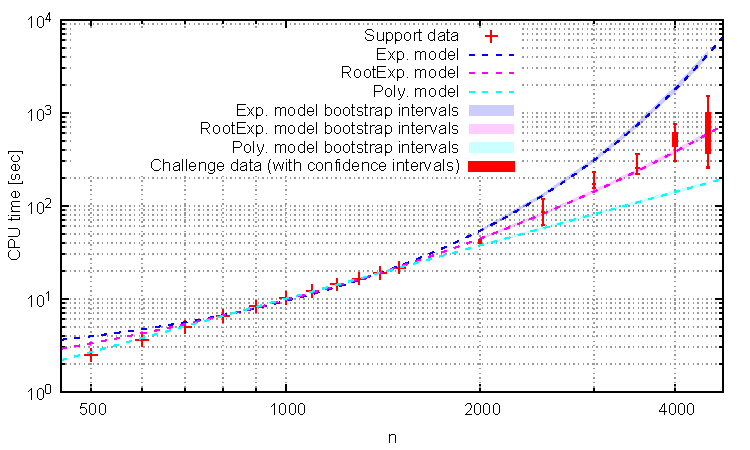
\includegraphics[width=0.7\textwidth]{EAX_fittedModels} \vspace{-5mm}

\par\end{centering}

\caption{Example output of ESA -- running times, fitted models and corresponding bootstrap confidence intervals.}\label{fig:ESA-fitted-models}
\end{figure*}

\item A figure showing the residues of the fitted models, which helps the user easily see trends in the residues of the fitted models, as illustrated in Figure~\ref{fig:ESA-fitted-residues}.
\begin{figure*}[t]
\noindent \begin{centering}
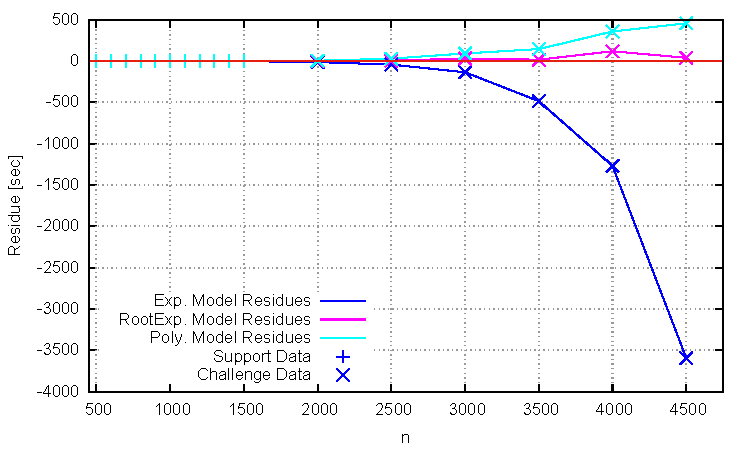
\includegraphics[width=0.7\textwidth]{EAX_fittedResidues} \vspace{-5mm}

\par\end{centering}

\caption{Example output of ESA -- residues of the fitted models}\label{fig:ESA-fitted-residues}
\end{figure*}


\item A table of bootstrap confidence intervals for all model parameters, which allows a user to assess the uncertainty in the fitted models and perhaps accept or reject hypotheses about whether or not empirical observations match theoretical expectations about an algorithm's scaling. An example is shown in Table~\ref{tab:ESA-bootstrap-paras}.
\begin{table}[t]
\begin{centering}
\caption{\label{tab:ESA-bootstrap-paras}Model confidence intervals example}
\scalebox{0.75}{%
\begin{tabular}{cc|cc}
\hline
Solver  & Model  & Confidence interval of $a$  & Confidence interval of $b$ \tabularnewline
\hline
\multirow{3}{*}{EAX} & Exp. & $\left[1.6182,1.6777\right]$ & $\left[1.0017,1.0018\right]$ \tabularnewline
 & RootExp. & $\left[0.23777,0.2565\right]$ & $\left[1.1218,1.1244\right]$ \tabularnewline
 & Poly. & $\left[1.6402\times10^{-5},2.1752\times10^{-5}\right]$ & $\left[1.8875,1.9281\right]$ \tabularnewline
\hline
\end{tabular}%
}\medskip{}

\par\end{centering}

%\caption{\label{tab:ESA-bootstrap-paras}Example output of ESA -- bootstrap confidence intervals for all model parameters.}
\end{table}

\item A table of medians and bootstrap confidence intervals for the support and challenge RMSE of each model, which provides more information about how well the models fit the data than Table~\ref{tab:ESA-fitted-models} by leveraging the bootstrap analysis, as illustrated in Table~\ref{tab:ESA-bootstrap-RMSE}.

\begin{table}[t]
\begin{centering}
\caption{Model RMSE example}\label{tab:ESA-bootstrap-RMSE}
\scalebox{0.75}{%
\begin{tabular}{cc|cc|cc}
\hline
 \multirow{2}{*}{Solver} & \multirow{2}{*}{Model} & \multicolumn{2}{c|}{Support RMSE}  & \multicolumn{2}{c}{Challenge RMSE} \tabularnewline & & Median & Confidence Interval & Median & Confidence Interval \tabularnewline\hline
\hline
\multirow{3}{*}{EAX} & Exp. & $1.0862$ & $\left[1.0286,1.1404\right]$ & $1577.3$ & $\left[1209.6,1801.1\right]$ \tabularnewline
 & RootExp. & $\mathbf{0.61754}$ & $\mathbf{\left[0.56284,0.67104\right]}$ & $\mathbf{71.045}$ & $\mathbf{\left[12.057,394.81\right]}$ \tabularnewline
 & Poly. & $0.15889$ & $\left[0.11768,0.2076\right]$ & $251.38$ & $\left[121.37,592.91\right]$ \tabularnewline
\hline
\end{tabular}%
}\medskip{}

\par\end{centering}

%\caption{Example output of ESA -- medians and bootstrap confidence intervals for support and challenge RMSE.}

\end{table}

\item Two tables, for each model, of bootstrap confidence intervals for
observed and predicted running times, one for support data and the
other for challenge data. These tables allow the user to easily identify which model predictions are weakly or strongly consistent with the observations through boldface and asterisks. An example for challenge data is illustrated in Table~\ref{tab:ESA-bootstrap-challenge}.
\begin{table*}[t]
\begin{centering}
\caption{Observed and predicted challenge confidence intervals example}
\label{tab:ESA-bootstrap-challenge}
\scalebox{0.75}{%
\begin{tabular}{ccccc}
\hline
\multirow{2}{*}{Solver} & \multirow{2}{*}{$n$} & Predicted confidence intervals & \multicolumn{2}{c}{Observed median run-time}\tabularnewline
 &  & RootExp. model  & Point estimates  & Confidence intervals\tabularnewline
\hline
\hline
\multirow{4}{*}{EAX} & 2000 & $\left[43.72,45.07\right]$ & $41.26$ & $\left[40.05,42.41\right]$ \tabularnewline
 & 2500 & $\mathbf{\left[80.21,83.7\right]}$ & $86.62$ & $\left[62.31,119.2\right]$ \tabularnewline
 & $\cdots$ & $\cdots$ & $\cdots$ & $\cdots$ \tabularnewline
 & 4500 & $\mathbf{\left[571.2,620.6\right]}$ & $\left[368.4,982.4\right]$ & $\left[257.9,1528\right]$ \tabularnewline
\hline
\end{tabular}%
}\medskip{}

\par\end{centering}

%Example output of ESA -- bootstrap confidence intervals for observed running times and predictions from the fitted root-exponential model for the support data (upper table) and the challenge data (lower table); ``...'' represents omitted lines analogous to those shown.
\end{table*}
 
\end{itemize}
A snapshot of the report generated by ESA using the default {\LaTeX}
template is shown in Figure \ref{fig:Snapshot-ESA-output}, the full report can be found at \url{www.cs.ubc.ca/labs/beta/Projects/ESA/samples/scaling\_EAX.pdf}. 
\begin{figure*}[t]
\begin{centering}
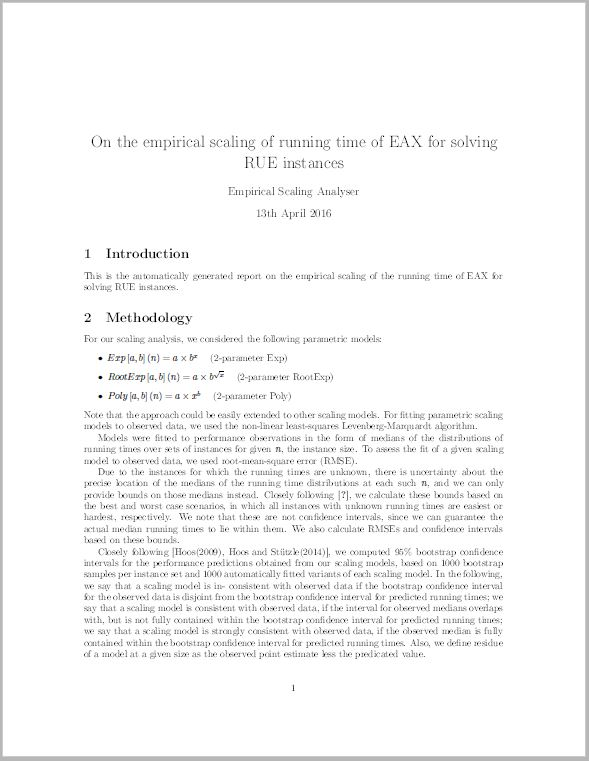
\includegraphics[width=0.48\textwidth]{ESA_output_1}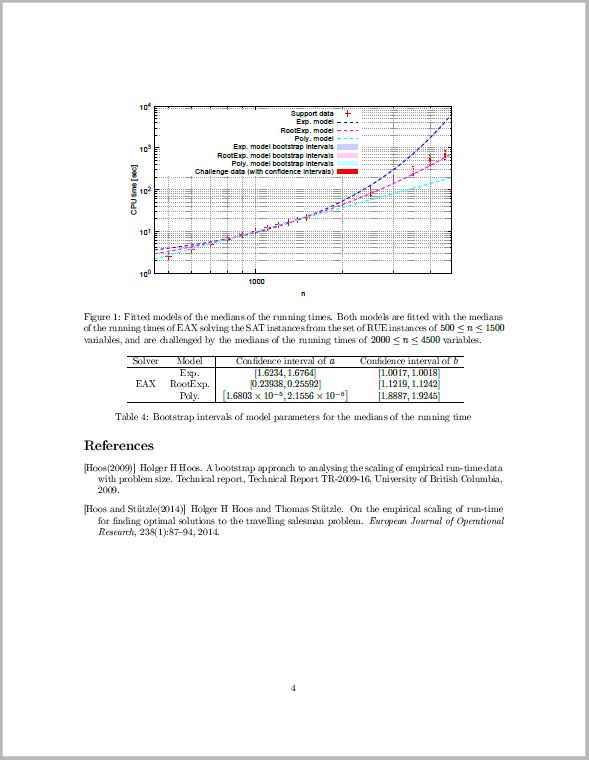
\includegraphics[width=0.48\textwidth]{ESA_output_2}
\par\end{centering}

\caption{A snapshot of the 7-page technical report generated by ESA.}\label{fig:Snapshot-ESA-output}
\end{figure*}


\section{Benchmark sets}
\label{sec:AA}

%HH: I'd make it clearer in this section intro that we proceed in two stages; first, we do "stress testing" (don't use those words), for which we need these benchmarks; then, we discuss "real-world" applications (TODO: YP)
In order to assess the quality of the results obtained by ESA in various situations, it is important to have complete control over the properties of the running time data set being used as input. In computing science, it is common practice to analyse theoretical properties of algorithms, such as the worst case running time complexity; however, since in practice the observed scaling may be much better than asymptotic worst-case bounds, we cannot rely on the theoretical properties of an algorithm to justify whether or not ESA has correctly identified the true empirical scaling. To this end, we have developed a general technique for producing approximately realistic running time data sets with known scaling properties.

Any artificially generated data set of running times should display to the greatest possible degree characteristics similar to those of realistic application scenarios. 
Towards this end, we simulated a randomized algorithm with three distinct sources of variability in running time: 
variance due to differences between problem instances (of the same size); variance in running times between multiple independent runs on the same problem instance; and changes in running times as a function of instance size.
To simulate the variance from independent runs on a single instance, we draw samples from an exponential distribution, parameterized to have a median running time equal to the desired running time for the instance. 
We chose to model the variance with an exponential distribution to closely resemble behaviour observed for a range of prominent stochastic local search algorithms for SAT~\cite{HooStu99}. 
Similarly, to determine the median running time for a given instance, we draw a sample from an exponential distribution with a prescribed median.
%HH: Can we justify this assumotion? I'd refer at least to observed high variability in (median) running times across insances of the same size ... (TODO YP)
Finally, to determine the median running time for a given instance size, we use a given scaling model mapping instance size to median running time.

As an example, assume we want to generate running times for a randomized algorithm with quadratic scaling on an instance of size $n = 1\,000$. 
First, we would pick the running time scaling model, e.g., $10^{-6} \cdot n^2$, and use it to compute the median running time for instance size $1\,000$ -- in this case $10^{-6} \cdot 1\,000^2 = 1$ (CPU seconds). 
Second, we draw a sample from an exponential distribution with median $1$. 
In this case, assume we draw a value of $0.83291$ (CPU seconds); this means that $0.83291$ is the median running time for that particular instance. 
Finally, if we want to simulate 3 independent runs of the algorithm on this instance, we would draw 3 samples from an exponential distribution with median $0.83291$.


\section{Stress testing}
\label{sec:Stress Testing}

There are many potential factors that could cause ESA to report misleading or incorrect results: for example, it could erroneously accept an incorrect scaling model because of misleading lower-order terms, or because the predicted confidence intervals are so large that any model fits the data. 
Clearly, the latter case is more benign than the first, but it is not always clear how to resolve the problem. 
%In many cases, more data is needed -- perhaps running times for more instance sizes, larger challenge instance sizes, more instances per size, or more independent runs per instance. 
%HH: <- this sentence is good, but doesn't fit into the flow here. (TODO - integrate elsewhere, e.g., end of section of conclusions)
%HH: new text:
To better understand the robustness and limitations of ESA, we conducted a series of carefully designed \emph{stress-testing experiments}.
Specifically, by varying properties of artificially generated benchmark sets of running time (see Section~\ref{sec:AA}), we studied the performance of ESA for a range of challenging situations.

%HH: You need to explain somewhere (perhaps here), which kind of stress tests you describe in this section, and which in the next. At the very least, because you mention lower-order terms above, you should make it clear that you are investigating the degree to which they cause issues in Section 6. (TODO)

We generated two data sets, using a polynomial and an exponential scaling model. For the polynomial model, we used $2.58\cdot 10^{-10} \cdot n^{3.37}$, which tended to fit some real running time data obtained from a TSP solver in preliminary experiments. 
We fitted the exponential model to data from the polynomial model, to make the two models as similar as possible. 
We generated running times for 21 instance sizes: 500, 600, ..., 1900, 2000, 2500, ..., 4500, and we used 16 support instance sizes, 5 challenge instance sizes, 500 instances per size and 10 independent runs per instance. 
We set ESA's parameters to their default values, using 1\,000 bootstrap samples and an alpha value of 95, and we studied the median running time of the per-instance medians. 
%HH: I am confused - does the following speak of the same instance set? I think not ... yet, no clear distinction is drawn ...
Since the instance sets are sampled from a probability distribution, we created a very large data set with 10\,000 instances per size and 100 independent runs per instance. 
This allowed us to perform 1\,000 independent runs of ESA on various sub samples of the original data set with the desired properties.

In the following, we provide only a high-level summary of our findings, and distill from these results generic advice on best-practices for using ESA. 
For a substantially more detailed discussion and presentation of the results, please see our online, supplementary material available at \url{http://www.cs.ubc.ca/labs/beta/Projects/ESA}~\todo{Not yet online (though ESA v1.1 is). Currently available at https://www.overleaf.com/6216557917nztjdzchjhxp}
%HH: <- TODO: put on-line before submission

%HH: All of the following should be a bit more concrete, without being significantly longer. Rather than giving vague statements, such as "say 10", refer to concrete examples of what you have seen. If we don't do this, giving details on the experimental setup (above) is useless, and we run a risk that reviewers simply aren't convinced. (TODO)

\textbf{What happens when we decrease the number of support instances per instance size?}
ESA can identify that the correct model fits the data even with a very small number of instances per size; however, this is because the size of the bootstrap confidence intervals for the fitted model predictions grows much more quickly than the size of the confidence intervals for the observed challenge statistics, \ie{}, all of the fitted models fit the data very well for small instance sets. In particular, we found that for extremely small numbers of support instances per size (say 10), the predicted confidence intervals were up to 3 or 4 orders of magnitude larger than the observed intervals (for the polynomial model on the polynomial data set), and up to 4 or 5 orders of magnitude larger than when 1\,000 instances were used per instance size.

\textbf{What happens when we decrease the number of support instance sizes?}
To our surprise, we observed that ESA reported far less false positives in this case than when we reduced the number of instances per instance size, relative to the total number of support instances available, eg., the root-exponential model was reported to tend to fit the data less than 20\% of the time for both the polynomial and exponential model when given as few as 3 support instance sizes, compared to just over 80\% of the time when given 16 support instance sizes, but only 20 instances per size -- a roughly comparable total number of support instances.

However, while this may seem like a good option for saving on computational expenses, we advise extreme caution when analyzing results with ESA that use very small numbers of support instance sizes. In particular, when ESA does report a false positive, it does so with predicted confidence intervals that are orders of magnitude smaller than in the case with less instances per instance size, which may lead the user to incorrectly assume that ESA's best-fit model accurately captures the true scaling. In real scenarios, we expect there to be an added challenge for ESA: coping with the effects of lower order scaling terms, which would likely significantly increase the probability that ESA will incorrectly classify the scaling when only a few support instances sizes are used. Furthermore, as we discuss in Section~\ref{sec:Lower Order Terms}, the best safeguard of which we are aware to combat against making incorrect assumptions due to lower order terms, is to look at the degree to which the model fits both the support and challenge data. When a very small number of support instance sizes are available, this type of safeguard becomes unavailable. 

\textbf{What happens when we reduce the number of independent runs per instance?}
Here we see the same sort of trend as when we reduced the number of instances per instance size; however, the decrease in confidence and the increase in false-positives are much more benign in this case. In particular, consider the decrease from 10 runs per instance to 1 run per instance, compared to the difference from using 500 instances per instance size to 50 instances per size. In both cases, we are decreasing the total number of algorithm runs by a factor of 10. However, the response in the size of the bootstrap intervals, and hence in ESA's interpretation of the model fit, is drastically different in the two cases. In particular, when 1 run per instance is performed the size of the predicted bootstrap interval for instance size 4\,500 is $1.7\cdot 10^4$, compared to when 50 instances per instance size are used, which resulted in a predicted bootstrap interval size of $7.4\cdot 10^5$ -- these numbers are different by a factor of 44. With such a striking difference it is clear that if the time required to collect all of the running time data is constrained, then the best option is to use very few independent runs per instance and to choose to instead use more instances per instance size if they are available.

\textbf{What happens when we increase the extrapolation distance?}
Overall, these results line up well with our intuition: the farther the extrapolation the higher the probability that ESA will correctly identify the true scaling and reject incorrect scaling. While this may seem an unsurprising result, it does indicate that the separation of the fitted models grows more quickly than the size of the predicted intervals, otherwise ESA's ability to distinguish between the models would not increase. As a result, increasing the extrapolation distance is one of the best ways to obtain more reliable and statistically significant results with ESA. Of course, it comes at the cost of the algorithm runs themselves requiring more running time. 

\textbf{What happens when we decrease the number of bootstrap samples ESA uses?}
We found that modifying this parameter had a mostly negligible effect on ESA's performance, which we found somewhat surprising when we used extremely small numbers of bootstrap samples (even as few as 20). Overall, the largest effect that we observed was a change in ESA's running time, which is roughly linear with the number of bootstrap samples. We believe that we would have observed more significant effects on ESA's performance had we also used less support data, so we still recommend to use at least 1\,000 bootstrap samples, since the cost is so small relative to performing additional algorithm runs. On the other hand, we observed no significant benefit to increasing this number either. 

%YP: Continue proof reading from here.

\section{Lower order terms}
\label{sec:Lower Order Terms}

One possible source of difficulty for ESA occurs when the underlying running time scaling contains lower order terms which initially compete with the true, asymptotic scaling. For example, an algorithm may scale asymptotically as an exponential; however, for small instance sizes the scaling may appear to be polynomial because the running times are being dominated by polynomial start-up costs incurred by initializing data structures. 

To investigate these effects we used running time data sets generated with two polynomial terms with degrees 2 and 5. For the degree 2 polynomial term we used the coefficient $9.6\cdot 10^{-7}$. To create three different data sets, we used three values for the degree 5 polynomial coefficient: $4.8\cdot 10^{-15}$, $4.8\cdot 10^{-16}$ and $4.8 \cdot 10^{-17}$. These values were chosen so that the transition occurs near the low, middle and high end of the instance sizes, respectively. The data sets contained 11 independent runs per instance with 1\,000 instances for each of the 21 instance sizes 500, 600, ..., 1\,900, 2\,000, 2\,500, ..., 4\,500. 

In addition, we ran ESA three times using three different values for the number of support instance sizes: 8, 12 and 16. In each case, all remaining instance sizes were used as challenge data. These experiments produced a total of nine different ESA reports which we examined in detail. 
We also provided ESA with a four parameter, two term polynomial model of the form $a\cdot n^b + c\cdot n^d$, to see if ESA could accurately fit four parameter models of the correct scaling class. 
In the following, we present a selected subset of the results that illustrates our main observations. 

\textbf{What happens when the transition is early?}
\begin{figure*}[t]
\centering
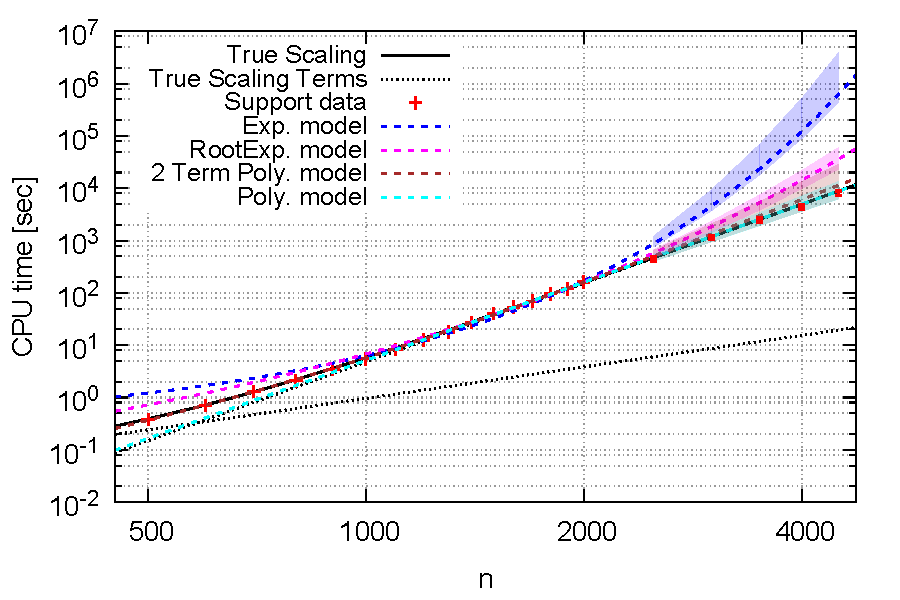
\includegraphics[width=0.7\textwidth]{fittedModels-2-5-14-16s.pdf}
\caption{\textbf{Early transition example:} generated using $4.8\cdot 10^{-15} \cdot x^5 + 9.6\cdot 10^{-7} \cdot x^2$ with 16 support instance sizes. \note{We'll need to decide whether or not we want colour figures. They cost extra, but you have to contact them to obtain a quote for the price. I think for these three figures in particular it would be nearly impossible to understand them without colour (and I'm not confident that I could make them legible without).}}
\label{fig:AA-competing-2-5-14-16s}
\end{figure*}
When the transition between terms occurs among the small support instance sizes, the fit of the single term model is able to capture the asymptotic scaling relatively accurately, \eg{}, see Figure~\ref{fig:AA-competing-2-5-14-16s}, where a polynomial model of degree 4.97 fits the challenge data very well. In comparison, the two term polynomial model provides a better fit for the small instance sizes, but yields larger predicted bootstrap intervals. For this model ESA fit a degree of 2.00 for one of the polynomial terms and a degree of 5.14 for the other, and reported that this model also fit the data very well. 

These results are positive, but we note that ESA does have some difficulty fitting the 4 parameter model. One indication is that higher-quality default parameter values are needed for the two term model than for single term models. Another sign can be seen by looking at the confidence intervals for the degrees of each term in the four parameter model, $[1.41,4.87]$ and $[4.77,6.26]$. These intervals are both larger than the single term model's interval and we see that they overlap, that is, in some cases the degrees were both large. This likely corresponds to a large support instance size outlier that caused ESA to over-fit. 

\textbf{What happens when the transition is mid?}
\begin{figure*}[t]
\centering
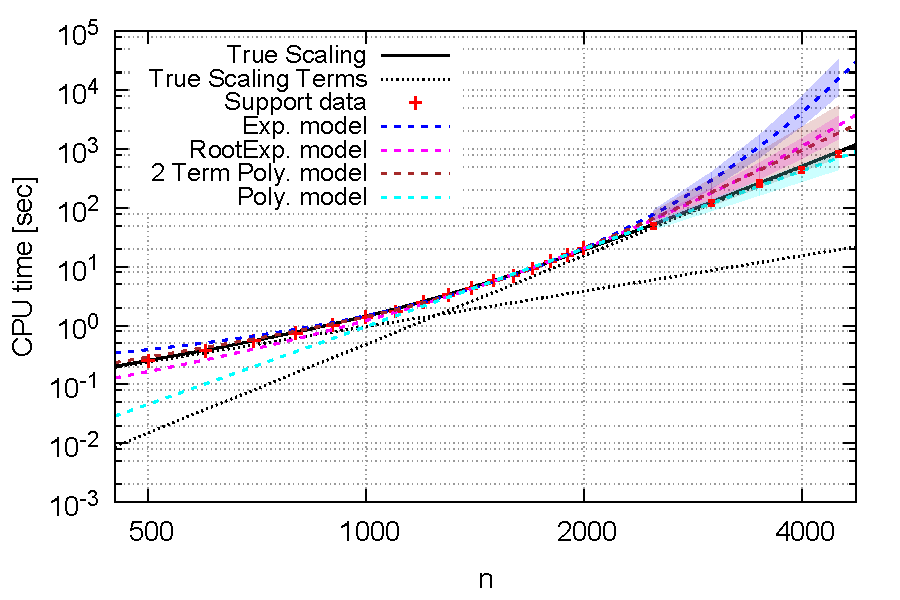
\includegraphics[width=0.7\textwidth]{fittedModels-2-5-15-16s.pdf}
\caption{\textbf{Mid transition example:} generated using $4.8\cdot 10^{-16} \cdot x^5 + 9.6\cdot 10^{-7} \cdot x^2$ with 16 support instance sizes.}
\label{fig:AA-competing-2-5-15-16s}
\end{figure*}
As the transition between the two terms moves closer to the large end of the support instance sizes, the quality of the ESA report starts to degrade. Overall, ESA is still able to do quite well as long as the location of the transition is completely covered by the support instance sizes, as seen in Figure~\ref{fig:AA-competing-2-5-15-16s}, where the predicted bootstrap intervals for both types of polynomial models capture the observed challenge data. The single term model is reported to ``fit the data very well'' despite that it does not quite capture the true degree of the asymptotic scaling in its interval $[4.00,4.74]$. On the other hand, the two term model, which is only reported to ``tend to fit the data'', does capture the true asymptotic scaling with the intervals $[1.50,2.30]$ and $[4.78,7.06]$. 

In this case, we also see that ESA had less trouble distinguishing between the two polynomial terms when fitting the two term polynomial model, since the bootstrap intervals for the degrees of the two terms are disjoint. However, we also see that the size of the predicted bootstrap intervals for the two term model has increased significantly. We believe this is because there are only a small number of instance sizes past the midpoint of the transition, hence there is less data to help ESA recover from the presence of a single outlier. When we decrease the number of support instance sizes (data not shown) we find that the predicted bootstrap intervals are similarly large for the two term polynomial; however, the single term model is unable to accurately capture the asymptotic scaling.

\textbf{What happens when the transition is late?}
\begin{figure*}[t]
\centering
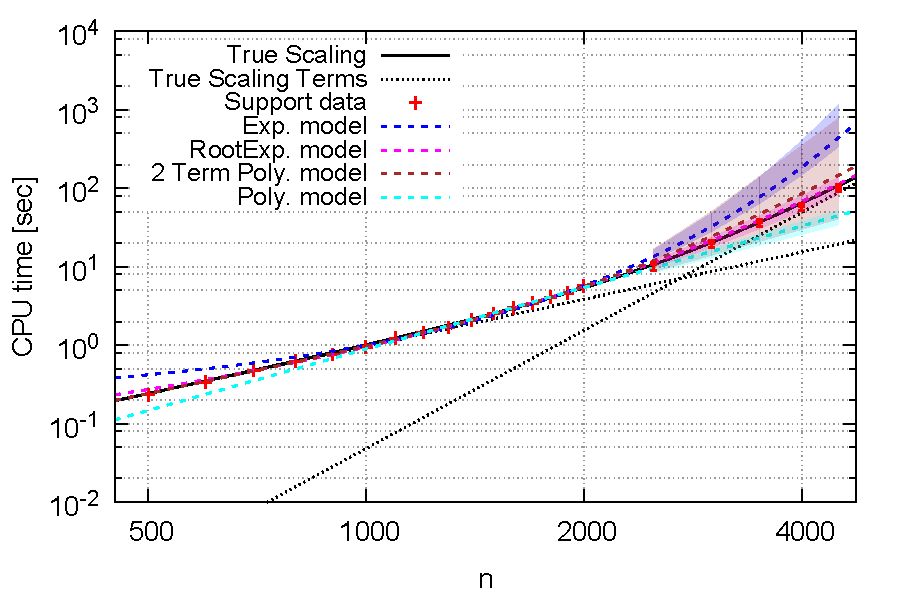
\includegraphics[width=0.7\textwidth]{fittedModels-2-5-16-16s.pdf}
\caption{\textbf{Late transition example:} generated using $4.8\cdot 10^{-17} \cdot x^5 + 9.6\cdot 10^{-7} \cdot x^2$ with 16 support instance sizes.}
\label{fig:AA-competing-2-5-16-16s}
\end{figure*}
The worst case scenario for ESA occurs when the transition between two competing terms happens after most or all of the support instance sizes, where ESA has little to no hope of correctly identifying the true asymptotic scaling. for an example of the worst-case behaviour, see Figure~\ref{fig:AA-competing-2-5-16-16s}, where the square-root exponential model appears to fit the data very well. On the positive side, at least ESA also identifies that the two term polynomial model fits the data very well. In practice, the safest course of action in this case is to collect more running time data -- in particular, larger challenge instance sizes -- and run ESA again. On the other hand, if this is not possible, a pragmatic user would be inclined to choose the square-root exponential model as the one that is the best fit, while keeping in mind that it may be an over-estimate for the true running time scaling. In fact, we can already begin to see that this is the case by examining the smallest support instance sizes, for which we can see that the curvature of the square-root exponential model is beginning to pull the model away from the observed running times -- a sign which may generalize to other scenarios where the best-fit model may not be accurately capturing the scaling due to lower-order terms. 

We also observed that the size of the predicted bootstrap intervals continues to increase for the four parameter model. This is even more clear for the case with only 12 support instance sizes (data not shown), where the size of the predicted bootstrap intervals is huge (roughly spanning five orders of magnitude). 
We also tried running ESA on this data set with only 8 support instance sizes; however, ESA was unable to complete the analysis. After several attempts at restarting ESA, we found that the Levenberg-Marquardt algorithm simply was unable to fit the four parameter model to the data -- even when the default fitting parameters were set to the true values for the running time scaling, the implementation of the Levenberg-Mardquart algorithm we used crashed. 

\textbf{What if we know something about the lower order terms?}
Practical applications of ESA to algorithms with competing terms may have known scaling for start-up costs, \eg{}, the initialization of a data structure may be known to have quadratic scaling. Hence we may be inclined to use a three parameter, two term polynomial model of the form $a\cdot n^b + c\cdot n^2$. 

We ran ESA again on each of the 9 scenarios; however this time we used the three parameter, two term polynomial model. Overall, the results did not change significantly. In a few cases the fit of the 3 parameter model was slightly better for the small instance sizes; however, it appeared to remain unchanged for the challenge instance sizes. We also observed that the predicted bootstrap intervals were both slightly smaller and located slightly higher in most of the scenarios. The only exception to this observation was for the function $4.8\cdot 10^{-15} \cdot x^5 + 9.6\cdot 10^{-7} \cdot x^2$ when ESA was run with 8 support instance sizes  (a mid transition scenario). We found that with the four parameter model the predicted bootstrap intervals were very large (comparable to those in Figure~\ref{fig:AA-competing-2-5-16-16s}); however, with the three parameter model they were substantially smaller (comparable to those in Figure~\ref{fig:AA-competing-2-5-15-16s}). 
Unfortunately, the Levenberg-Mardquart algorithm was still unable to successfully complete for all 1000 bootstrap samples of the $4.8\cdot 10^{-17} \cdot x^5+ 9.6\cdot 10^{-7} \cdot x^2$ data set when only 8 support instance sizes were used. 


\section{Successful applications}
\label{sec:Successful Applications}

During the development of ESA, earlier versions were used in several projects to analyze the empirical scaling of various high-performance algorithms \cite{Mu15}. These early applications provided interesting results, as well as valuable insights that helped us improve ESA subsequently. 
%HH: I added the following, but this doesn't quite set the stage for what follows. Please modify / amend this to make it clear what we summarise in the following and why (e.g., why don't we outline the first, published applications?) - TODO
In the following, we outline the findings obtained from these earlier applications.

A first use of ESA extended our earlier scaling analysis of six prominent SAT solvers on random phase-transition 3-SAT instances \cite{MuHoo15} to two classes of random 4-SAT instances. This work, described in detail in Section~5.4 of \cite{Mu15}, yielded several interesting results: for phase-transition instances, exponential (for BalancedZ) or root-exponential models (for the other solvers) usually characterize best the running times of SLS-based, incomplete SAT solvers, while DPLL-based, complete solvers demonstrate scaling behaviour well characterized by exponential models; for solving a class of less-constrained instances believed to be intrinsically challenging, we showed that WalkSAT/SKC and kcnfs, two widely studied SAT solvers, scale significantly better than on phase-transition random instances, in that a polynomial model best describes the observed performance scaling.

In another application of ESA, we improved previous scaling results for the state-of-the-art inexact TSP solvers, EAX and LKH~\cite{DubEtAl15}, with additional data; details on these results are found in Section 6.3 in~\cite{Mu15}. ESA determined that EAX scales root-exponentially, best described by a model of the form $a\cdot b^{\sqrt{n}}$ with $b\approx 1.123$, as shown in Figure \ref{fig:ESA-fitted-models}. For LKH, we also observed evidence for root-exponential scaling, but we cannot rule out a polynomial model (see Figure \ref{fig:Fitted-models-LKH}). We also used ESA to analyze the time required by the state-of-the-art complete TSP solver, Concorde, to find optimal solutions without proving optimality. A root-exponential model of the form $a\cdot b^{\sqrt{n}}$, with $b \approx 1.25$ as illustrated in Figure~\ref{fig:Fitted-models-concorde}, was found to best describe the scaling behaviour. Besides, ESA produced substantial evidence that both EAX and LKH scale better than Concorde for finding optimal solutions to RUE instances.
\begin{figure*}[t]
\noindent \begin{centering}
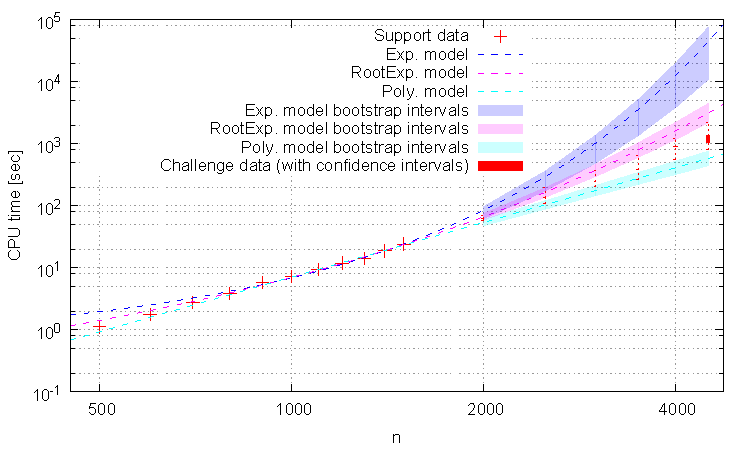
\includegraphics[width=0.7\textwidth]{LKH_fittedModels}  \vspace{-5mm} 
% \includegraphics[width=0.7\textwidth]{fittedModels}

\par\end{centering}

\caption{Scaling models for median running times of LKH for finding optimal solutions to RUE instances.}\label{fig:Fitted-models-LKH} 
\end{figure*}
\begin{figure*}[t]
\noindent \begin{centering}
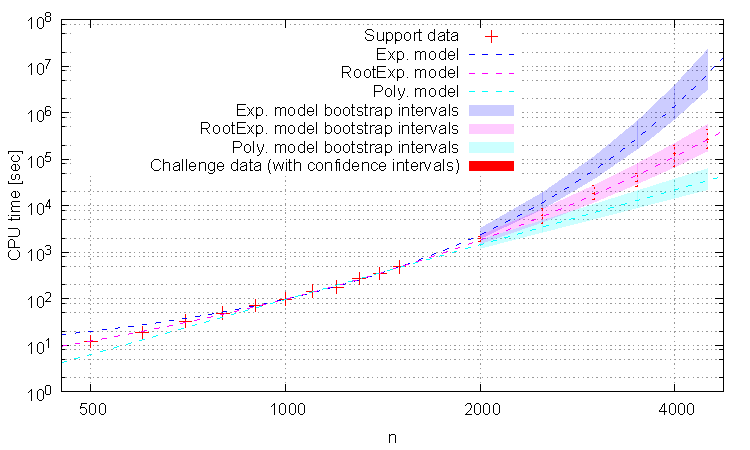
\includegraphics[width=0.7\textwidth]{concorde_fittedModels}  \vspace{-5mm}
\par\end{centering}

\caption{Scaling models for the medians of the running times for Concorde to find optimal solutions of RUE instances. }\label{fig:Fitted-models-concorde} 
\end{figure*}


Finally, using ESA, we investigated the impact of parameter settings and automated algorithm configuration on the performance scaling of inexact TSP algorithms~\cite{MuEtAl16}. For EAX, algorithm configuration helps improve the scaling, which can be further improved by adapting the population size with instance size. In particular, we achieved an $\approx1.13$-fold improvement in the median running time for EAX to solve RUE instances of size $n=4\,500$ and expect the improvement to be even more significant for larger instances. For LKH, we observed significant impact of parameter settings on performance scaling, but the state-of-the-art algorithm configurator SMAC tends to overfit the running times for smaller instances and thus produces configurations for which LKH scales worse.

%HH: The following explanation comes late. This may be OK if you fix the issue pointed out near the beginning in a compelling way, but currently, it doesn't work. (TODO: fix above and/or here)
The results in this section are from previous work done using an earlier version of ESA. The only change to the methodology underlying ESA since these results were obtained is the addition of the nested bootstrap sampling procedure to handle independent runs of a randomized algorithm on an instance.  Unfortunately, the only remaining copy of the original data are files containing the per-instance medians, so we were unable to directly compare the newest version of ESA to the old on the original data. To compare with the older version of ESA, we reran EAX on the same instance set using 11 independent runs per instance. Overall, the results are qualitatively very similar to those previously found. However, we did find that the sizes of the bootstrap intervals for the observed challenge instances increased by 4.2\% on average, where the size of an interval is defined to be the upper bound divided by the lower bound. Similarly, the size of the intervals for the root-exponential model that best describes the running times increased by an average 
%HH: Really? A factor of 0.1% (TODO: fix - see my revised wording above)
factor of 0.1\%. 
%(note that there were significantly more instances available for each support instance size than for the  challenge instance sizes, hence the uncertainty of the fitted models is much smaller than the uncertainty of the challenge instance sizes). 
%By properly handling the uncertainty from independent runs of a randomized target algorithm ESA is less likely to obtain false-negative results by rejecting the correct scaling model class; however, in our experiments we have not yet observed a scenario where using the old version of ESA rejected a scaling model when the current one fails to do so.

\section{Conclusions and future work}
\label{sec:Conclusion}

In this work, we introduced the empirical scaling analyzer (ESA), an automated tool for analyzing the empirical scaling of algorithm performance with input size. ESA can fit multiple models on the input running time data and generate results in the form of technical reports. These reports contain easy-to-read figures and tables as well as automatically generated interpretations. We also presented new methodology to appropriately handle the variance between independent runs of a randomized algorithm and a novel method for automatically interpreting the scaling analysis results.  

We presented a rigorous analysis of ESA's performance when subjected to challenging scenarios. In particular, we found that increasing the number of instances used per instance size is a more cost-effective means of increasing the power of ESA's statistical tests than increasing the number of independent runs per instance. Based on our results, we caution against using small numbers of support instance sizes, since this can make it challenging or impossible to identify whether or not lower order terms or outliers have cased ESA to incorrectly classify the algorithm's scaling. From our experience, we recommend to use around 11 support instance sizes, though the exact number needed will vary by scenario. 
We found that ESA can correctly classify an algorithm's asymptotic scaling when lower order terms are present, provided that the transition between the two models occurs early enough in the support sizes. However, increasing the number of parameters in a parametric model to capture both the lower order terms and the asymptotic scaling substantially increases the size of the predicted bootstrap intervals and causes ESA to have more trouble fitting the models. Furthermore, ESA has significant trouble and can incorrectly classify the scaling if the transition between the models occurs after the large support instance sizes. 

Overall, we have found that ESA is able to perform well in most scenarios. Unlike theoretical running time analysis, there is always the risk that a lower order term is initially dominating the running time, and hence larger instance sizes are needed to accurately identify the true asymptotic scaling. Nevertheless, empirical scaling analysis plays a key role in characterizing and understanding the behaviour of high-performance algorithms for important problems. This is particularly true for scenarios where the observed performance of algorithms exceeds the expectations provided by a worst case analysis or in cases where theoretical assumptions about the expected behaviour of an algorithm may not hold true for real-world instances. The methodology underlying ESA is widely applicable to problems and algorithms where running time data can be gathered for various instance sizes. ESA provides an easy and convenient way to apply empirical scaling analysis to algorithms of interest. Thus, we believe that ESA will prove to be a useful tool for researchers studying both the empirical and theoretical scaling behaviour of algorithms, and we hope that ESA will promote and enhance such studies.

There are several directions for future improvements of ESA. In particular, it would be interesting to automatically select models from a large family of functions based on input data. This could also facilitate fitting of models with lower-order terms. One possible approach towards this end involves repeated fitting of models, first on the original data, then on the residues, in order to obtain a model with several terms. %Extended in this way, ESA could become easily applicable to an even broader range of algorithms with little human input, and may produce even more interesting results. Future work could also extend ESA to perform sensitivity analysis on each of the support instance sizes. In this way, users could be alerted if it appears that the presence of a single outlying data point is causing the fitted models to incorrectly capture the running time scaling. 
Another possible extension, could be to completely remove ESA's requirement that instances be grouped by size, allowing users to simply input a collection of instances with varying sizes. Such an extension would enable users to apply ESA to an even broader range of applications, since it may not always be possible to collect instances grouped by size. We believe that many users of ESA may be motivated to find upper or lower bounds on the running times required to solve very large instances. To this end, future extensions of ESA could be developed that fit tight bounds on the running time scaling to provide users with such estimates.

Another interesting avenue of study is the performance of ESA when used to analyze the scaling of polynomial-time algorithms. Preliminary results indicate that such algorithms tend to have significantly less noise in their running times than the heuristic, $\mathcal{NP}$-hard algorithms that have been the primary subject of our study so far. Very small bootstrap intervals can provide new challenges for ESA that will need to be overcome in future extensions, since all of the fitted models tend to be rejected. The introduction of tight, upper and lower bounds to ESA's methodology may also be a method for resolving this challenge.

In addition, we are currently working on uses of ESA in the development of automated algorithm configuration procedures for better scaling behaviour. Such procedures could make automated configuration even more applicable to real-world situations, as problem instances of practical interest can take a long time to solve. Automated configuration usually requires many runs of the given target algorithm with different parameter settings, which can make it infeasible to run a configuration procedure directly on large, challenging instances.
Previous work on the problem of automatically configuring algorithms for improved performance scaling has focused on generic protocols for using existing configurators~\cite{StyEtAl12,StyHoo13}. 
An alternative consists of incorporating empirical scaling analysis, as performed by ESA, more directly into algorithm configuration. Unfortunately, the current version of ESA requires running time data for many problem instances of different sizes,
which can take a long time to produce. Thus, it will be important to design a way to reduce the time, possibly by leveraging previously fitted models, \eg{}, by integrating Bayesian methods into empirical scaling analysis, with a previous model acting as the prior for model fitting. This could lead to an enhanced version of ESA that could then be integrated into a future configuration procedure.


\begin{acks}
YP was supported by an NSERC Vanier Scholarship. HH acknowledges funding through an NSERC Discovery Grant, CFI JLEF funding and startup funding from Universiteit Leiden. \todo{Did Zongxu have funding that needs to be added here? HH: I don't think so.}
\end{acks}

\bigskip
% TODO: will be deleted and changed to Acknowledgements in the final version


\noindent
\footnotesize
\textbf{Note to reviewers:} 
Two of the three case-studies mentioned
are unpublished and only appear in the M.Sc. thesis of Mu. \note{Do we actually even need this at all? I think there are enough contributions to this paper that the ``successful applications of ESA'' could almost be moved into a section call ``related work'', that combines it with some of the material from the introduction. HH: IMO, successful applications are very important, because otherwise, we only talk about results on artificial data, showing limitations. But the note to reviewers is not needed if these results are correctly framed (with pointers to the thesis) in Section 7.}




%\begin{figure}[t]
%\includegraphics{}
%\caption{Figure caption.}\label{f1}
%\end{figure}

%\begin{table*}
%\caption{} \label{t1}
%\begin{tabular}{lll}
%\hline
%&&\\
%&&\\
%\hline
%\end{tabular}
%\end{table*}

%%%%%%%%%%% The bibliography starts:

%%%%%%%%%%%%%%%%%%%%%%%%%%%%%%%%%%%%%%%%%%%%%%%%%%%%%%%%%%%%%
%%                  The Bibliography                       %%
%%                                                         %%
%%  ios1.bst will be used to                               %%
%%  create a .BBL file for submission.                     %%
%%                                                         %%
%%                                                         %%
%%  Note that the displayed Bibliography will not          %%
%%  necessarily be rendered by Latex exactly as specified  %%
%%  in the online Instructions for Authors.                %%
%%                                                         %%
%%%%%%%%%%%%%%%%%%%%%%%%%%%%%%%%%%%%%%%%%%%%%%%%%%%%%%%%%%%%%


%\nocite{*} 
% if your bibliography is in bibtex format, use those commands:
\bibliographystyle{ios1}           % Style BST file.
\bibliography{scaling}        % Bibliography file (usually '*.bib')

% or include bibliography directly:
%\begin{thebibliography}{0}
%\bibitem{r1} F. Author, Information about cited object.
%
%\bibitem{r2} S. Author and T. Author, Information about cited object.
%\end{thebibliography}

\end{document}
